\section{int\_pulse\_lut}

clear\_int的下一级是一个组合逻辑,使用LUT4来实现的。

\textbf{int\_pulse\_lut.v}
\begin{vcode}
 // synthesis translate_off 
 defparam int_pulse_lut.INIT = 16'h0080 ;
 // synthesis translate_on 
 LUT4 int_pulse_lut ( 
 .I0(t_state),
 .I1(clean_int),
 .I2(int_enable),
 .I3(active_interrupt),
 .O(int_pulse ))/* synthesis xc_props = "INIT=0080"*/;
\end{vcode}



这个LUT4的初始值是0x0080。用卡诺图表示如下:

\textbf{karnaugh graphic}
\begin{textcode}
||= bit(3210) =||= xx11 =||= xx10 =||= xx00 =||= xx01 =||
||         11xx||     0  ||     0  ||     0  ||     0  ||
||         10xx||     0  ||     0  ||     0  ||     0  ||
||         00xx||     0  ||     0  ||     0  ||     0  ||
||         01xx||     1  ||     0  ||     0  ||     0  ||
\end{textcode}



很容易写出逻辑关系式:

\textbf{logic}
\begin{vcode}
assign out = !bit3 & bit2 & bit1 & bit0;
\end{vcode}

现在可以改写为rtl风格的代码:

\textbf{int\_pulse\_lut\_rtl.v}
\begin{vcode}
always@(t_state or clean_int or int_enable or active_interrupt)
begin
    if (!active_interrupt && int_enable && t_state && clean_int)
        int_pulse = 1;
    else
        int_pulse = 0;
end
\end{vcode}



这个int\_pulse\_lut逻辑用于开启和忽略中断信号。

同样用Synplify综合PicoBlaze得到的lut内部结构也是这样的

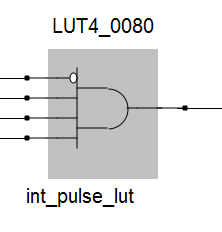
\includegraphics{int_pulse_lut}

